\section{\emph{rag}, a Ruby Autograder for ESaaS}

\texttt{rag} is actually a collection of three different autograding
``engines'' based on three open source testing
tools:
\begin{enumerate}

\item RSpec is a unit-testing and
BDD/TDD framework descended from XUnit, but which exploits Ruby's
flexible syntax to embed a unit-testing DSL in Ruby that results in very
readable tests.  

\item Cucumber allows
integration-level tests or user stories~\cite{user-stories} to be
expressed in plain prose, using regular expressions to match each step
of such a test to a block of code that sets up preconditions (\texttt{Given}), stimulates
the system (\texttt{When}), or checks postconditions (\texttt{Then}) as
appropriate; our code blocks are in Ruby, but the Cucumber framework
itself is language-agnostic.  

\item Capybara~\uf{jnicklas.github.io/capybara}
provides a Ruby-embedded DSL for interacting with Web-based
applications.
One can trigger actions on a web page such as filling in form fields
or clicking a button, and use XPath~\cite{xpath} to examine the
response page delivered by the server.
Capybara actions can either run in the same process as the app being
tested, or when used in conjunction with the Mechanize
library~\footnote{\url{https://rubygems.org/gems/mechanize}; based on
  the older Perl library of the same name.}, can trigger these actions
against a remote application, allowing black-box testing.

\end{enumerate}




c.	Student expderience. Submit files online, wait a bit, receive numerical score + feedback.

d.	RSpecGrader

coverage

internal structure of code, eg checking if students used correct
abstraction 



e.	FeatureGrader


In mutation testing, invented by George Amman and Jeff Offutt (cite), a
testing tool mutates the program under test by introducing random logic
errors that do not result in syntax or compilation errors.  If no test fails
in the presence of an introduced error, there is a gap in test
coverage.  We use a variant of this approach to grade an
assignment in which students are required to write integration-level
tests for an existing SaaS application.

Students use the Cucumber tool (cite) to create these tests.
Cucumber allows integration and acceptance tests to be formulated in
stylized plain text, as Figure~\ref{fig:cucumber} shows.
Since a SaaS application is being tested, black-box integration tests
must stimulate the SaaS application in the same way that
a human being user a Web browser would.
Depending on the testing environment, Cucumber can do this in one of
three ways.  The first uses a built-in browser simulator that hooks
directly into 
the Rails application server, and thus can only be used
with application stacks that use this server and that do not rely on
JavaScript.  The second is using Webdriver (formerly 
Selenium) to control a real browser via a now-standard remote-control
API (cite Webremote).  The third, which we use, uses a Ruby library called
Mechanize\footnote{Based on the Perl library of the same name.} to
direct requests to an application deployed on  a remote server.  


f.	CIGrader - like AWAT [cite]. can assess full-stack GUI apps interactively. Mentioned as Future  Directions area in both Douce and Ihantola surveys.

g.	Summary table: grader types, types of assignments they grade, and how students submit work



\begin{figure}
  \begin{minipage}{0.45\textwidth}%
  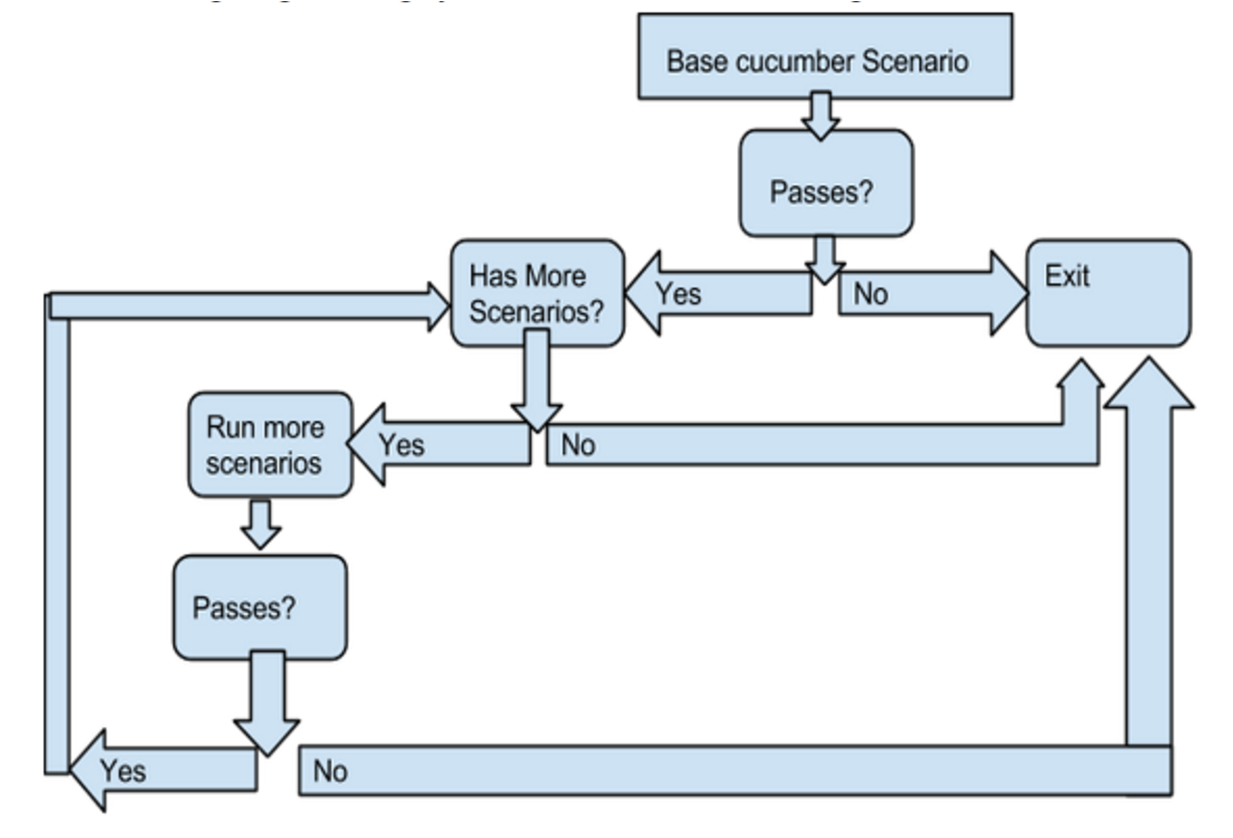
\includegraphics[width=\textwidth]{figs/feature_grader.pdf}%
  \end{minipage}%
  \begin{minipage}{0.55\textwidth}%
  \lstinputlisting{figs/feature_grader_example.yml}%
  \end{minipage}
  \caption{\label{fig:cucumber}%
FeatureGrader workflow and example YAML file.  In this case if Step1-1 passes,
Step1-3 will be run next.  Earlier steps must be less restrictive than
later steps (if the earlier step fails, there should be no way that a later one could pass).
\texttt{failures} are the two student-provided Cucumber scenarios that \emph{should fail} when
run because of mutations (bugs) inserted in the app.
}
\end{figure}
